
\begin{figure}[H]
  \centering
  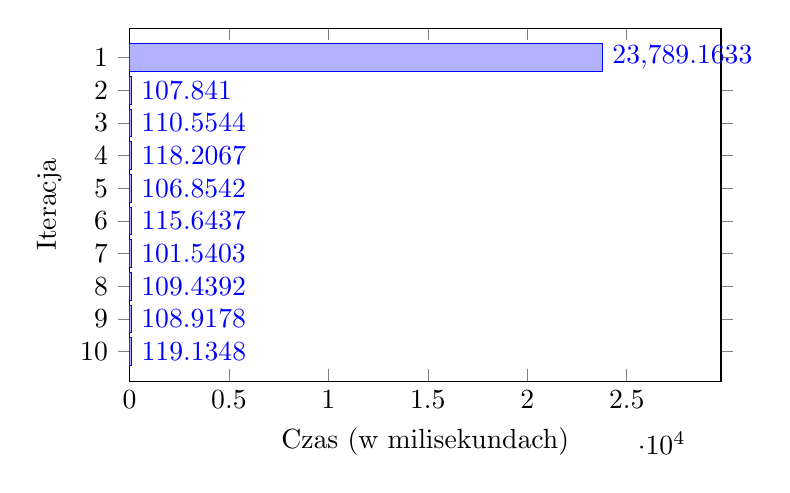
\begin{tikzpicture}
  
    \begin{axis} [
      xbar = .05cm,
      nodes near coords,
      nodes near coords style={
        /pgf/number format/precision=4,
      },
      xmin = 0,
      ytick = data,
      enlarge x limits = {value = .25, upper},
      symbolic y coords = {10,9,8,7,6,5,4,3,2,1},
      xlabel=Czas (w milisekundach),
      ylabel=Iteracja,
      width=0.75\textwidth,
      height=0.5\textwidth
    ]
    
      \addplot coordinates {(23789.163300037384,1) (107.841000020504,2) (110.55440002679825,3) (118.20670002698898,4) (106.85420000553131,5) (115.64370000362396,6) (101.54030001163483,7) (109.43919998407364,8) (108.91780000925064,9) (119.13480001688004,10)};
      
    \end{axis}
  
  \end{tikzpicture}
  \caption{Wynik testów przykładu 7 [\ref{lst:wydajnosc-przyklad-p-7}]}
  \label{fig:wynik-przyklad-6}
\end{figure}
